\documentclass[12pt, letterpaper, twocolumn]{article}
\usepackage[margin=1.0in]{geometry}
\usepackage{fontspec}
%\usepackage{unicode-math}
\setmainfont{Arial}
%\DeclareMathVersion{bhitc}
%\setmathfont[version=normal]{Arial}
\usepackage{fancyhdr}
\setlength{\headheight}{14.5pt}
\usepackage{graphicx}
\usepackage{caption}
\captionsetup[figure]{font=small}
\usepackage{amsmath}
\usepackage[]{siunitx}
\usepackage[style=numeric,sorting=none]{biblatex}
\addbibresource{references.bib}
\pagestyle{fancy}
\fancyhf{}
\lhead{Hannah W. Richards}
\rhead{University of Alabama}
\rfoot{\thepage}
\hyphenation{GAMMA-SPHERE}

\begin{document}

% title
\begin{center}
\textbf{Determining Yields of Fragment Pairs from the Spontaneous Fission of Californium-252}
\end{center}

% introduction
\noindent\textbf{Introduction}\\
About $3.1$ percent of californium-252 ($^{252}$Cf) nuclei undergo spontaneous nuclear fission,~\footnote{The remaining $96.9$ percent of nuclei $\alpha$-decay to $^{248}$Cm, which then follows a decay chain whose analysis was not part of this study.} in which the nucleus splits into two daughter nuclei,~\footnote{whose atomic numbers sum to that of ($_{98}$Cf)} followed by a number of neutrons evaporated (also known as the ``neutron channel'' number). Usually, only about $4$ neutrons are evaporated~\cite{osti_15053}, but an unexpectedly high yield of decays that evaporate $8$, $9$, and $10$ neutrons have been observed when barium ($_{56}$Ba) and molybdenum ($_{42}$Mo) are produced as daughter nuclei~\cite{PhysRevC.62.041601}. My role in this study was to determine the uniqueness of this case; my goal was to verify whether any other daughter nuclei element pairs were also capable of evaporating a high number of neutrons. I studied two element pairs: tellurium ($_{52}$Te) and palladium ($_{46}$Pd), and strontium ($_{38}$Sr) and neodymium ($_{60}$Nd) using $\gamma$-ray spectroscopy data taken of $^{252}$Cf with the GAMMASPHERE~\cite{LEE1990c641} detector array.

\vspace{0.125in}
% methods
\noindent\textbf{Methods}\\
I exploited the structure of the studied nuclei to measure how frequently certain isotope pairs of daughter fragments were produced. Under the nuclear shell model, nucleons~\footnote{neutrons and protons} occupy certain ``shells,'' or levels with specific energies, much like electrons do in the atom. When a nucleon descends an energy level, it emits a high energy photon ($\gamma$-ray) of energy equal to the difference in the energies of the final and initial levels. This process is called $\gamma$ decay. When a nucleus is at its lowest energy state, it is said to be in the ground state; otherwise, it is in an excited state.
Because each nuclear isotope has a unique series of levels and level transitions, the energies of $\gamma$-rays can be used as ``fingerprints'' for identifying specific isotopes (see Figure~\ref{fig:levels}). Of particular interest to me were the $\gamma$-rays emitted when nuclei decay to the ground state. Virtually all daughter nuclei from spontaneous fission begin in excited states; therefore, they must emit a ground state transition $\gamma$-ray at some point as they undergo $\gamma$ decay. Counting the number of ground state transition $\gamma$-rays is a standard method for determining the yields of specific isotopes in a decay process.~\footnote{A small number of daughter fragments will be produced in the ground state already, but their effect is negligible for this study.}

% figure 1
\begin{figure}[ht]
    \centering
    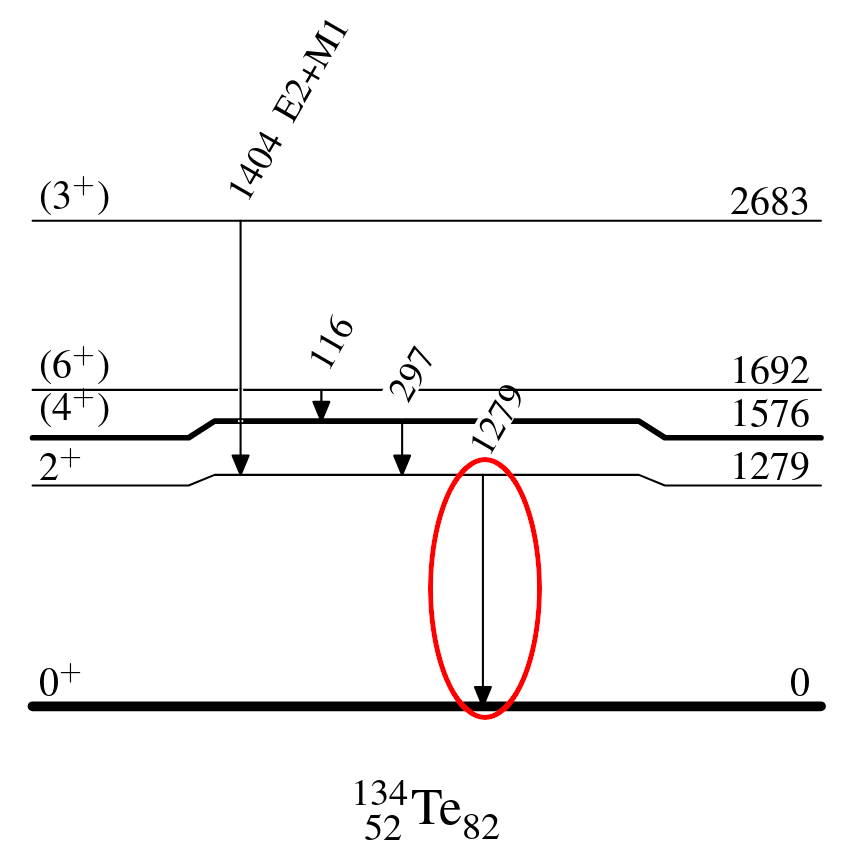
\includegraphics[width=0.4\textwidth]{img/level_scheme.png}
    \caption{The level scheme of $^{134}$Te, which shows all the discovered energy levels and transitions seen in this nuclear isotope. Circled in red is its ground state transition.}
    \label{fig:levels}
\end{figure}

To determine the yields of isotopes produced as daughter pairs in the decay, I had to add an additional layer of complexity to the measurements. I used coincidence counting, in which I chose, or ``gated on,'' the ground state transition of one daughter isotope, then measured the intensities of $\gamma$-ray peaks that were emitted at the ground state transition energies of its possible partner isotopes within a $1$~\si{\micro\second} coincidence window (see Figure~\ref{fig:spectrum}). From the figure, note that most intense peak belongs to $^{114}$Pd, indicating that it was produced in coincidence with $^{134}$Te more often than any other Pd isotope was. This is expected because $4$ neutrons must have been evaporated from these two isotopes, as the total number of neutrons between these two isotopes is $4$ fewer than in $^{252}$Cf. Deviating from $^{114}$Pd, one can see the intensities of the peaks drop, to the point where neutron channels of $9$ and $10$ are immeasurably small, if they exist at all. To perform my measurements, I used the software suite RadWare~\cite{RADFORD1995297}, which has utilities for gating on energies and measuring the intensities of $\gamma$-ray peaks.~\footnote{The intensity of a peak is the area underneath a normal distribution fit of the peak.}

% figure 2
\begin{figure}[ht]
    \centering
    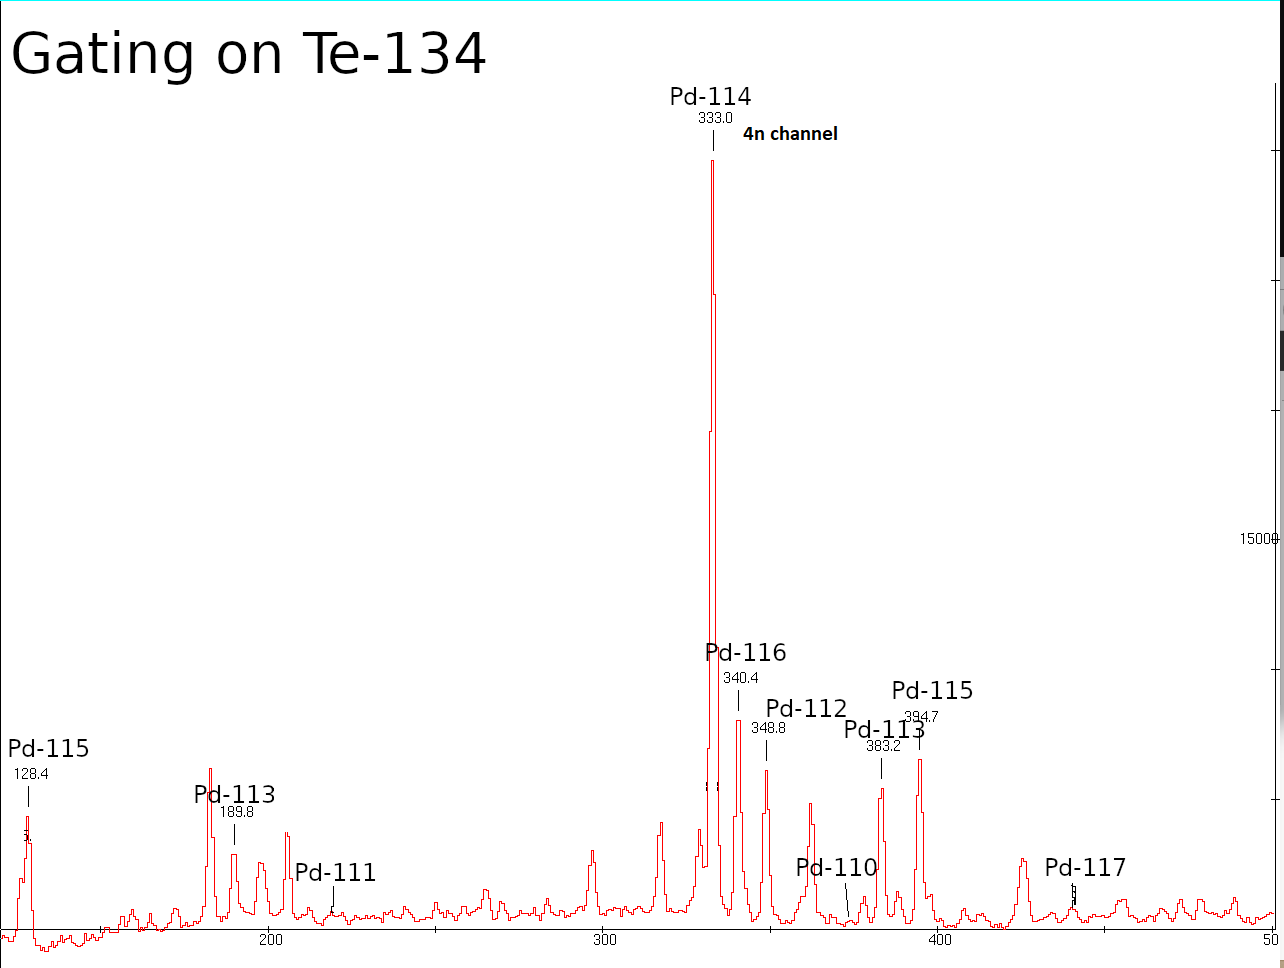
\includegraphics[width=0.49\textwidth]{img/spectrum_labeled.png}
    \caption{A gamma ray spectrum after coincidence counting on the ground state transition energy of $^{134}$Te. Labeled are the peaks of ground state transition energies of Pd isotopes.}
    \label{fig:spectrum}
\end{figure}

Complicating the process, some isotopes have multiple ground state transitions, such as $^{115}$Pd in Figure~\ref{fig:spectrum}. Each of these transitions has to be measured separately, with their results combined to obtain a total measurement for the isotope.

\vspace{0.125in}
% results
\noindent\textbf{Results}\\
After gating on each isotope of a daughter element and measuring the ground state transition peaks of the partner isotopes, I calculated the yields for each measured isotope pair using a script I wrote in Python. The calculations included correcting the measurement for the efficiency of the GAMMASPHERE detector~\cite{EnhongPhDThesis}, scaling for each isotope, and correcting for the internal conversion coefficient according to the \textit{BrIcc} database~\cite{KIBEDI2008202}.
I tabulated the yields in a matrix, which I then normalized and scaled according to calculations in Reference~\cite{WAHL19881} to obtain the absolute yields. My final yields matrices for the two studied element pairs are seen in Figures~\ref{fig:Te_yields} and \ref{fig:Nd_yields}.

% figure 3
\begin{figure}[ht]
    \centering
    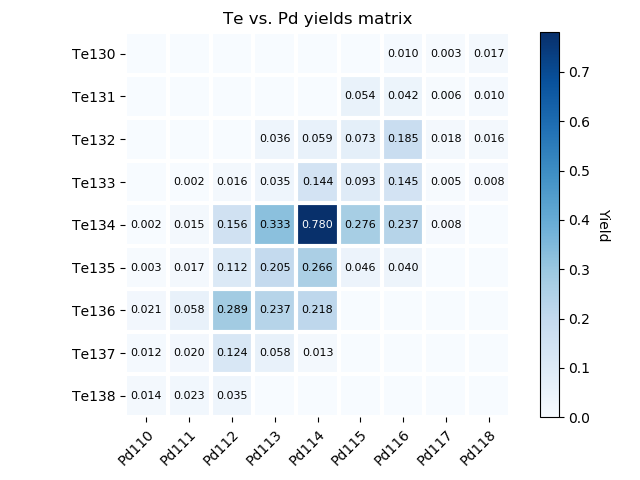
\includegraphics[width=0.49\textwidth]{img/yields_matrix_heatmap.png}
    \caption{The yields matrix for the element pair Te and Pd. On the horizontal axis are isotopes of Pd, and on the vertical, Te. The highest yields are in the center and along the diagonal of the matrix, indicating that the $4$ neutron channel was usually the highest, with zero yields seen for very high neutron channels (upper left corner).}
    \label{fig:Te_yields}
\end{figure}

% figure 4
\begin{figure}[ht]
    \centering
    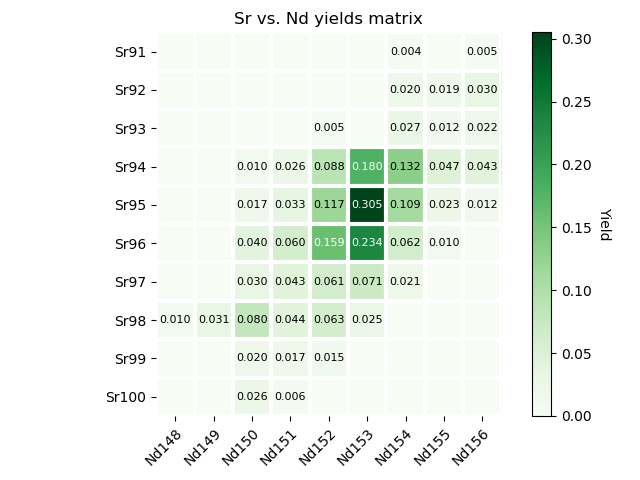
\includegraphics[width=0.49\textwidth]{img/nd_yields_matrix_heatmap.png}
    \caption{Similar plot seen in Figure~\ref{fig:Te_yields}, but for the other studied element pair, Sr and Nd. We can draw the same conclusion that the $4$ neutron channel usually had the highest yields, and there was no evidence for very high neutron yields as well.}
    \label{fig:Nd_yields}
\end{figure}

% figure 5
\begin{figure}[ht]
    \centering
    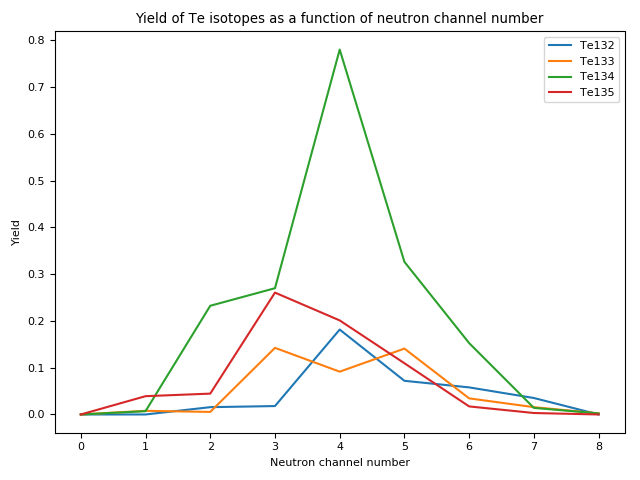
\includegraphics[width=0.49\textwidth]{img/neutron_channel.png}
    \caption{A plot of yields against the neutron channel number for select isotopes of Te, taken directly from the yields matrix (Figure~\ref{fig:Te_yields}). Note that the highest yields are clustered around $3$ or $4$, and become very small by $7+$.}
    \label{fig:channel}
\end{figure}

\vspace{0.125in}
\noindent\textbf{Conclusion}\\
There is no evidence for high neutron channel yields for my studied element pairs (see Figure~\ref{fig:channel}), unlike what was seen in the case of the Ba and Mo fragment pair. This supports the hypothesis that the Ba and Mo case is truly unique in the spontaneous fission of $^{252}$Cf, in that it is capable of evaporating up to $10$ neutrons. A possibility as to why this can occur is that a highly energetic, hyperdeformed $^{144}$Ba nucleus is produced immediately after scission;~\footnote{the splitting of the $^{252}$Cf nucleus} however, more research must be done to determine the exact cause of this anomaly.

\vspace{0.125in}
\noindent\textbf{Future Studies}\\
Continuing my study of nuclear decays, I am further broadening my research experience with the EXO-200 project, a search for a hypothetical form of exotic nuclear decay called neutrinoless double beta decay. Through this work, I am developing additional skills such as machine learning, optimization, and detector design---all valuable for any experimental physics project. Moreover, I intend to complete another research experience for undergraduates (REU) in a different nuclear or neutrino physics project, such as MicroBooNE, over the Summer of 2019.
%I would like to thank Vanderbilt University's Physics REU program. US DOE Grant No. DE-FG05-88ER40407 and NSF Grant No. 1560035.
%\nocite{*}
%\vspace{0.25in}
\newpage
\noindent\textbf{References}
\printbibliography[heading=none]

\end{document}
